\begin{figure*}[t]
    \centering
    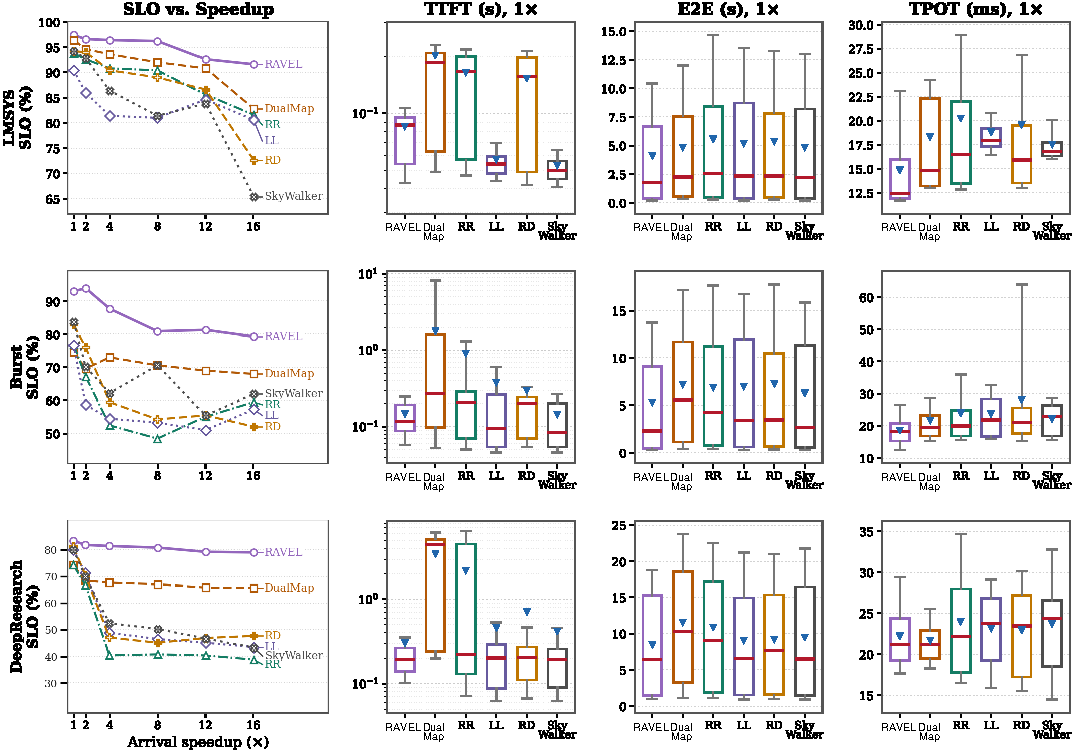
\includegraphics[width=\textwidth]{figures/end_to_end.pdf}
    \caption{
RAVEL preserves higher request-level SLO attainment as offered load increases.
Rows correspond to LMSYS, Burst, and DeepResearch.
The first column varies arrival speedup from $1\times$ to $16\times$; the
remaining columns report TTFT, end-to-end latency, and TPOT distributions at
$1\times$ load.
RAVEL consistently achieves the highest SLO attainment across the evaluated
workloads and loads, without requiring uniformly lower values of every
individual latency metric.
}
    \label{fig:main-results}
\end{figure*}

\section{Evaluation}
\subsection{Experimental Setup}
\label{sec:eval:setup}

\paragraph{Testbed and replay.}
We deploy five Qwen3-1.7B serving replicas across three clusters in a
2/2/1 configuration.  Each replica runs on an NVIDIA GeForce RTX~4090 GPU
with bfloat16 precision using vLLM~0.8.5.post1 (V0).
The final experiments use physical WAN transport rather than synthetic
latency injection; measured directed inter-cluster RTTs range from
10.1 to 37.9\,ms.
Table~\ref{tab:eval-setup} summarizes the common serving configuration.
All policies use the same hardware, topology, and base vLLM configuration;
RAVEL's TBT-aware local control is part of the system evaluated in
Section~\ref{sec:eval:mechanism}.

We replay requests \emph{open-loop}.  For an arrival-rate speedup $s$, we
scale trace inter-arrival times by $1/s$, so control-plane overhead cannot
backpressure the offered load.
We evaluate $1\times$, $2\times$, $4\times$, $8\times$, $12\times$, and
$16\times$ arrival rates, with 500 requests in every
policy--workload--load cell.
Before formal measurement, we warm all backends using the same execution
path.  Before each cell, we reset the prefix cache on every replica,
preventing cached state from carrying across policy comparisons.

\begin{table}[t]
\centering
\small
\caption{Evaluation testbed and serving configuration.}
\label{tab:eval-setup}
\begin{tabular}{@{}ll@{}}
\toprule
\textbf{Dimension} & \textbf{Configuration} \\
\midrule
Model               & Qwen3-1.7B \\
GPU                 & NVIDIA GeForce RTX 4090 \\
Precision           & bfloat16 \\
Serving engine      & vLLM 0.8.5.post1 (V0) \\
Deployment          & 5 replicas / 3 clusters (2/2/1) \\
Network             & Physical WAN \\
Inter-cluster RTT   & 10.1--37.9\,ms (directed) \\
Max. sequences      & 64 per replica \\
Max. batched tokens & 16,384 \\
Prefix caching      & Enabled \\
Chunked Prefill     & Enabled \\
Requests per cell   & 500 \\
Arrival speedup     & $1,2,4,8,12,16\times$ \\
\bottomrule
\end{tabular}
\end{table}

\paragraph{Workloads.}
We evaluate three workload regimes that expose different forms of contention
in geo-distributed serving.
\emph{LMSYS} contains heterogeneous conversational requests with diverse
prompt and response sizes.
\emph{Burst} uses the same 500 request contents as LMSYS but replaces their
arrival timestamps with BurstGPT timestamps.
This controlled construction isolates short-horizon arrival contention from
changes in the request-content distribution.
\emph{DeepResearch} is derived from multi-stage, completion-oriented
workflows.  We flatten branch requests by arrival time and evaluate the first
500 branch requests using request-level completion SLOs; the selected trace
does not define a workflow-level task SLO.
For DeepResearch, RAVEL's semantic output profile is constructed exclusively
from the designated training split and never uses the realized output of an
evaluation request.
Together, the workloads cover heterogeneous conversational traffic,
transient burst contention, and sustained completion-oriented demand.

\paragraph{SLOs.}
We use the JITServe-style heterogeneous-SLO construction implemented by our
evaluation runner.
The base budgets are 0.8\,s for TTFT, 80\,ms for TBT, and 8\,s for
end-to-end completion, with a request-specific multiplier from
$1\times$ to $4\times$.
For LMSYS and Burst, the released class-assignment procedure produces
181 LATENCY, 301 THROUGHPUT, and 18 COLLECTIVE requests in each
500-request trace (seed 42); DeepResearch branch requests are COLLECTIVE.
A LATENCY request succeeds only if its TTFT and every measured TBT satisfy
their respective budgets.
THROUGHPUT and COLLECTIVE requests instead succeed when their end-to-end
latency satisfies the corresponding completion budget.

\paragraph{Baselines.}
We compare RAVEL against five routing policies.
\emph{Round Robin (RR)} is stateless and distributes incoming requests
across serving replicas in round-robin order.
\emph{Least Load (LL)} tracks the number of outstanding requests at each
replica and routes each new request to the replica with the smallest
outstanding-request count.
\emph{Random (RD)} independently selects a serving replica at random for
each incoming request.
\emph{DualMap} jointly considers cache affinity and serving load and
rebalances traffic when affinity-driven placements become hotspots.
\emph{SkyWalker} performs locality-aware cross-region load balancing,
preferring available local capacity and redirecting requests when local
replicas become saturated while preserving prefix locality.
All policies replay identical request records over the same serving topology
and base engine configuration; each baseline uses only the state prescribed
by its routing policy.

\paragraph{Metrics.}
Our primary metric is \emph{request-level SLO attainment}, i.e., the
fraction of requests satisfying the class-specific success criteria above.
We additionally report time to first token (TTFT), time per output token
(TPOT), and end-to-end request latency to separate application-level SLO
outcomes from individual latency components.
For LATENCY requests, we additionally report TBT violations when analyzing
streaming performance.
All evaluated cells complete all 500 requests, and SLO misses remain in the
denominator.




\subsection{End-to-End Performance}
\label{sec:eval:e2e}

Figure~\ref{fig:main-results} summarizes RAVEL's end-to-end performance
across the three workload regimes.
The first column reports request-level SLO attainment as the offered load
increases from $1\times$ to $16\times$.
The remaining columns show the distributions of TTFT, end-to-end latency,
and TPOT at nominal load.
Together, these results characterize RAVEL's SLO attainment under increasing
contention and its latency behavior at nominal load.

\textbf{RAVEL sustains higher SLO attainment under load.}
RAVEL achieves the highest request-level SLO attainment across all three
workloads and every evaluated arrival rate.
The separation is particularly pronounced in several high-contention
settings.
At $16\times$ load, RAVEL attains 91.6\% of request SLOs on LMSYS,
compared with 82.8\% for the best-SLO baseline, DualMap;
79.2\% on Burst, compared with 62.0\% for SkyWalker; and
64.2\% on DeepResearch, compared with 47.6\% for RD.
These correspond to gains of 8.8, 17.2, and 16.6 percentage points,
respectively.
RAVEL therefore retains substantial advantages even when offered load
creates severe contention for serving capacity.

The contrast between LMSYS and Burst provides a controlled view of this
contention.
Burst preserves the same request contents as LMSYS and changes only their
arrival timestamps.
RAVEL's larger advantage on Burst therefore coincides with greater
short-horizon arrival contention rather than a change in the prompt or
response distribution.
The DeepResearch results further show that RAVEL's gains extend beyond mixed
interactive traffic to sustained completion-oriented demand.

\textbf{RAVEL improves SLO attainment while maintaining competitive
latency.}
At nominal load, RAVEL's TTFT, end-to-end latency, and TPOT distributions
remain competitive with the baselines across all three workloads.
Its SLO gains under stress are also accompanied by favorable P95 latency.
At $16\times$ load, RAVEL achieves both higher request-level SLO attainment
and lower P95 TTFT and P95 end-to-end latency than the best-SLO baseline for
each workload.
For example, on Burst, RAVEL reduces P95 TTFT from 8.70\,s to 2.68\,s and
P95 end-to-end latency from 28.68\,s to 18.78\,s relative to SkyWalker,
while increasing SLO attainment from 62.0\% to 79.2\%.
These results highlight the distinction between optimizing a single latency
statistic and maximizing class-specific request-level SLO attainment.

These end-to-end results establish RAVEL's performance benefit but do not
attribute it to individual mechanisms.
Section~\ref{sec:eval:mechanism} next isolates pre-handoff revisability and
RAVEL's SLO-specific execution controls.

\begin{figure*}[t]
    \centering
    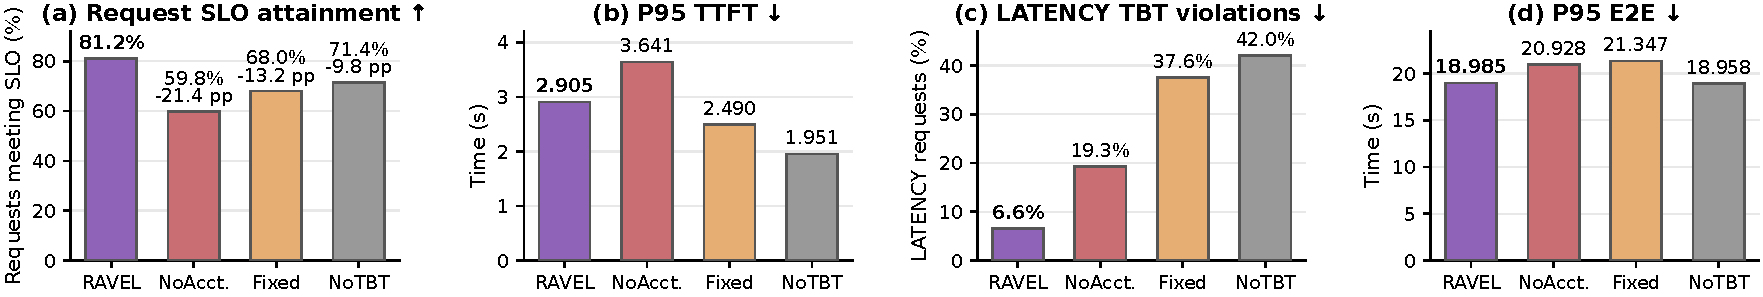
\includegraphics[width=\textwidth]{figures/mechanism_breakdown.pdf}
    \caption{
\textbf{Mechanism breakdown on Burst at $12\times$ load.}
\emph{FixedPlacement} retains immediate demand accounting but disables
pre-handoff reassignment; \emph{NoTBTGuard} retains Router-side RAVEL
placement but disables the local TBT-aware Chunked-Prefill guard.
We report (a) request-level SLO attainment, (b) P95 TTFT,
(c) the fraction of LATENCY requests with at least one TBT violation, and
(d) P95 end-to-end latency.
Both pre-handoff revisability and local TBT protection materially contribute
to RAVEL's SLO gains.
}
    \label{fig:mechanism-breakdown}
\end{figure*}
\subsection{Mechanism Breakdown}
\label{sec:eval:mechanism}

We next isolate the mechanisms behind RAVEL's end-to-end gains using the
Burst workload at $12\times$ load, where short-horizon contention is strong
while the request contents remain identical to LMSYS.
Figure~\ref{fig:mechanism-breakdown} compares full RAVEL with two ablations:
\emph{FixedPlacement}, which preserves immediate prospective demand
accounting but prevents a tentative replica assignment from changing before
engine handoff, and \emph{NoTBTGuard}, which preserves the global RAVEL
routing policy but disables the local TBT-aware Chunked-Prefill guard.
Each variant processes the same 500-request trace.
The TBT-violation metric is computed over the 181 LATENCY requests in that
trace.

\textbf{Pre-handoff revisability materially improves SLO attainment.}
Freezing the initial tentative placement reduces request-level SLO attainment
from 81.2\% to 68.0\%, a 13.2 percentage-point drop
(Figure~\ref{fig:mechanism-breakdown}a).
Importantly, FixedPlacement still accounts arrived demand immediately, so
later requests observe the load created by earlier tentative assignments.
What it removes is the ability to act on newly revealed demand by revising
those earlier assignments.
The resulting degradation therefore shows that demand visibility alone is
insufficient: earlier placements must remain revisable while they are still
under Router control.
This effect is also visible in streaming performance, where the LATENCY TBT
violation rate increases from 6.6\% under RAVEL to 37.6\% under
FixedPlacement (Figure~\ref{fig:mechanism-breakdown}c).

The result is particularly notable because FixedPlacement does not have worse
TTFT.
Its P95 TTFT is 2.49\,s, compared with 2.91\,s for RAVEL
(Figure~\ref{fig:mechanism-breakdown}b), yet it satisfies substantially fewer
complete request SLOs.
This reinforces the distinction between optimizing one latency component and
preserving the joint SLO constraints that determine whether a request
actually succeeds.

\textbf{Global placement and local TBT protection address complementary
sources of SLO loss.}
Disabling RAVEL's local TBT guard lowers request-level SLO attainment from
81.2\% to 71.4\%, a 9.8 percentage-point reduction.
The clearest change is in the LATENCY requests: their TBT violation rate rises
from 6.6\% to 42.0\%.
At the same time, NoTBTGuard has a lower P95 TTFT than RAVEL
(1.95\,s versus 2.91\,s) and nearly identical P95 end-to-end latency
(18.96\,s versus 18.99\,s).
The degradation is therefore concentrated in the streaming constraint that
the guard is designed to protect rather than in a broad increase in
completion latency.
These results show that selecting an appropriate replica globally is not
sufficient by itself; the local serving path must also bound Prefill
interference in accordance with activ e TBT requirements.

Together with the LateBind experiment in Figure~\ref{fig:motivation}, these
ablations separate the two parts of RAVEL's core design.
Late binding delays commitment but also delays regional demand attribution,
whereas FixedPlacement makes demand visible immediately but removes
pre-handoff revisability.
RAVEL combines both properties: arrived demand influences subsequent
placement decisions immediately, while tentative assignments remain
changeable until engine handoff.


\begin{figure}[t]
    \centering
    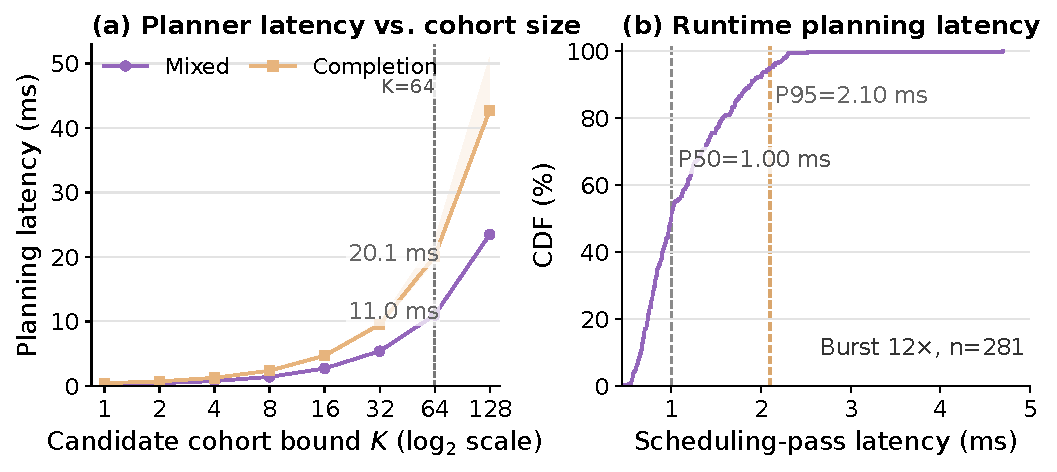
\includegraphics[width=\columnwidth]{figures/planner_overhead.pdf}
    \caption{
    \textbf{RAVEL control-plane scalability and runtime overhead.}
    (a) Planner latency versus candidate-cohort size for the mixed-traffic
    WorkYield and completion OnTimeSet planners; the dashed line marks the
    mixed-path bound $K=64$.
    (b) CDF of scheduling-pass latency in a 500-request Burst run at
    $12\times$ load.
    The runtime median/P95 are 1.00/2.10\,ms, while the mean/P95 candidate
    cohort sizes are 3.65/7 requests.
    }
    \label{fig:planner-overhead}
\end{figure}

\subsection{Control-Plane Scalability and Overhead}
\label{sec:eval:overhead}

We finally evaluate whether RAVEL's pre-handoff replanning can operate on the
online serving timescale.
Figure~\ref{fig:planner-overhead} separates two questions.
First, we measure how planner latency scales with the size of the candidate
cohort using states derived from the Burst and DeepResearch traces.
For each planner and cohort size, we run five warm-up iterations followed by
50 measured repetitions on an isolated CPU.
Second, we instrument an end-to-end Burst run at $12\times$ load and report
the distribution of planning latency observed during actual execution.

\textbf{Bounded replanning keeps multi-request planning tractable.}
Figure~\ref{fig:planner-overhead}a varies the candidate cohort from 1 to
128 requests for both RAVEL planning paths.
Planning cost increases with cohort size, with the completion planner
consistently more expensive because it additionally considers protected-set
replacement and deferred-request retries.
At RAVEL's normal cohort bound of $K=64$, the median planning latency is
10.99\,ms for the mixed planner and 20.10\,ms for the completion planner;
their P95 latencies are 11.18\,ms and 22.61\,ms, respectively.
Even when the replayed cohort is increased to 128 requests, median latency
remains 23.47\,ms for mixed traffic and 42.75\,ms for completion traffic.
These measurements show the role of the cohort bound: RAVEL does not require
multi-request optimization over the entire Router-owned queue, but confines
the more expensive placement computation to an explicitly bounded working
set.

\textbf{Online planning usually operates far below the configured bound.}
Figure~\ref{fig:planner-overhead}b reports all 281 planning passes from a
500-request Burst run at $12\times$ load.
The median planning latency is 1.00\,ms, with P95 and P99 latencies of
2.10\,ms and 2.30\,ms, respectively; the maximum observed pass takes
4.70\,ms.
The reason actual costs are substantially below the $K=64$ replay point is
that online cohorts are typically small: the mean cohort size is 3.65,
the P95 is 7, and the maximum observed cohort is 9.
Thus, the configured bound protects the control plane against unusually
large reversible sets, while the common online path replans only a small
number of requests at a time.

Overall, these results show that preserving pre-handoff placement
revisability does not require continuously solving a large global assignment
problem.
RAVEL instead performs bounded multi-request replanning when additional
information becomes available, and the measured online planning path remains
at millisecond-scale latency under the evaluated burst workload.
